\documentclass[11pt]{amsart}
\usepackage{geometry}                % See geometry.pdf to learn the layout options. There are lots.
\geometry{letterpaper}                   % ... or a4paper or a5paper or ... 
%\geometry{landscape}                % Activate for for rotated page geometry
%\usepackage[parfill]{parskip}    % Activate to begin paragraphs with an empty line rather than an indent
\usepackage{graphicx}
\usepackage{amssymb}
\usepackage{epstopdf}
\usepackage{hyperref}
\usepackage{acronym}
\usepackage{booktabs}
\DeclareGraphicsRule{.tif}{png}{.png}{`convert #1 `dirname #1`/`basename #1 .tif`.png}
\acrodef{WSN}[WSN]{Wireless Sensor Network}
\acrodef{IDE}[IDE]{Integrated Development Environment}
\acrodef{RGG}[RGG]{Random Geometric Graph}
\acrodef{UI}[UI]{User Interface}
\acrodef{JRE}[JRE]{Java Runtime Environment}
\newtheorem{definition}{Definition}
\title{Backbone Determination of Wireless Sensor Networks\\Manual}
\author{Zizhen Chen\textsuperscript{\copyright}}
\begin{document}
\maketitle
\begin{abstract}
\acp{WSN} have been the focus of intense research during the past few years because of their potential to facilitate data acquisition and scientific studies\cite{werner2006deploying}. Lack of a fixed infrastructure and dynamic network topology make the routing problem one of the most challenging issues in the \ac{WSN} area. One popular solution is forming a virtual backbone that forwards the packets. This algorithm engineering work graphically presents a procedure of backbone determination of various \ac{WSN} geometries. The whole work is implemented via a software sketchbook Processing that is both a programming language and an \ac{IDE} built for visual arts\cite{reas2007processing}. This article is a manual of using the implemented graphic program.
\end{abstract}
\section{Introduction}
\acfp{WSN} are composed of inexpensive autonomous electronic sensors distributed over regions where the sensors communicate with each other wirelessly. Sensors are typically thrown in an unattended and random manner on the area to be monitored. Wireless communication allows the formation of flexible networks, which can be deployed rapidly over wide or inaccessible areas. Nowadays, WSNs emerge as an active research area in which challenging topics involve energy consumption, routing algorithms, selection of sensor locations, and so forth\cite{carlos2016wireless}.

In a \ac{WSN} of a given topology (as Figure \ref{fig:wsn} shows), the sensor information is usually collected then forwarded to a base station known as sink node.
\begin{figure}[htp]
	\centering
	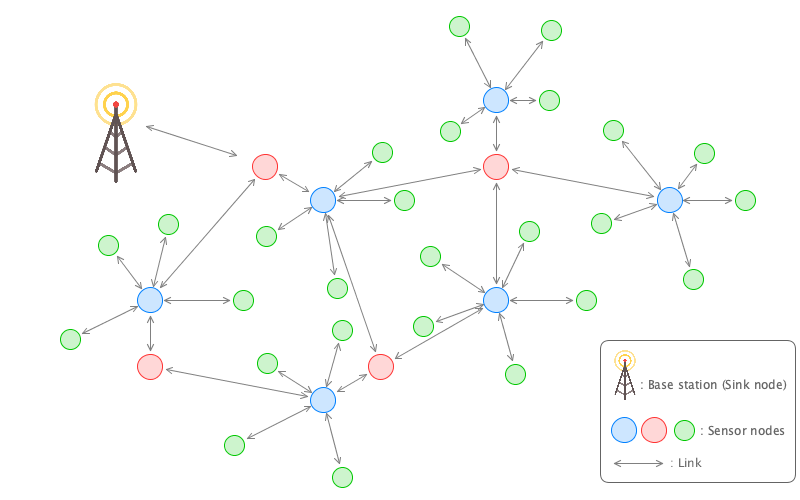
\includegraphics[width=.8\linewidth]{images/WSN.png}
	\caption{Wireless Sensor Network}
	\label{fig:wsn}
\end{figure}
The need to gather data from all sensors in the network imposes constraints on the distances between sensors, so an efficient routing is required if large number of sensors are involved. Routing through only a connected subset of nodes (called ``virtual backbone”) in a WSN is one solution\cite{al2008efficient,mahjoub2009experimental,chen2017bipartite}. As only nodes in the virtual backbone (e.g. the blue and red nodes in Figure \ref{fig:wsn}) forward packets or perform in-network services, other nodes can spend more time in a low-power idle mode. Therefore, a virtual backbone can simplify the routing process and reduce the overall network energy consumption. It also has other functions, such as transmission scheduling, broadcasting, and localization\cite{wang2005distributed}. We use an \ac{RGG} and cluster-based control structure to model a \ac{WSN}. \ac{RGG} denoted $G(n,r)$ chooses random n locations of nodes uniformly and independently in a region and two nodes are connected by an edge if they are within a Euclidian distance less than a certain value $r$\cite{dall2002random}. Cluster-based control structure allows a more efficient use of resources especially when a network consists of a large number of sensors\cite{carlos2016wireless}. Clustering consists in partitioning a network into a number of clusters each is achieved by grouping nodes inside a certain transmission area (in the case of an \ac{RGG}, it is a disc of radius $r$). A cluster is a locally connected group of nodes with a leading node (known as ``cluster-head") from which each of the other nodes (known as ``slave nodes") is one hop away. Forwarding information packets among cluster-heads requires a group of nodes as routing relays. We call such group of nodes a ``relay set” and accordingly, the set of cluster-heads is called a ``primary set”. The union of a primary set and a relay set forms a virtual backbone.
\begin{definition}
	A \textbf{virtual backbone} of a \ac{WSN} of cluster-based control structure is a connected subset of nodes composed of a primary set of cluster-heads and a relay set of routing relays. Backbone network provides a path for the exchange of information between sensor nodes and sink nodes.
\end{definition}
In Figure \ref{fig:wsn}, each blue node is a cluster-head that controls its adjacent green nodes as slave nodes, and each red node is a routing relay to its adjacent blue nodes. The blue and red nodes form a virtual backbone routing the network’s information to the base station.

This program partitions a \ac{WSN} modeled as an \ac{RGG} into a limited number of densely packed disjoint backbones. Each backbone is a subgraph that is composed of a pair of primary and relay set.
\section{Prerequisites}
\subsection{Platform}
Processing is developed based on Java, so there is no platform limitation unless some rare platform does not support \ac{JRE}. We exported the program to Windows (64-bit), macOS and Linux. They are available at \url{http://lyle.smu.edu/~zizhenc/Project}. If you are using other platforms, the source code are located on GitHub: \url{https://github.com/zizhenc/WSN}. However, the program does require a mouse and a keyboard as input devices. It also supports single touch behavior if you have a touch screen.
\subsection{Screen Size}
Figure \ref{fig:view} shows a typical view of the program. 
 \begin{figure}[htp]
	\centering
	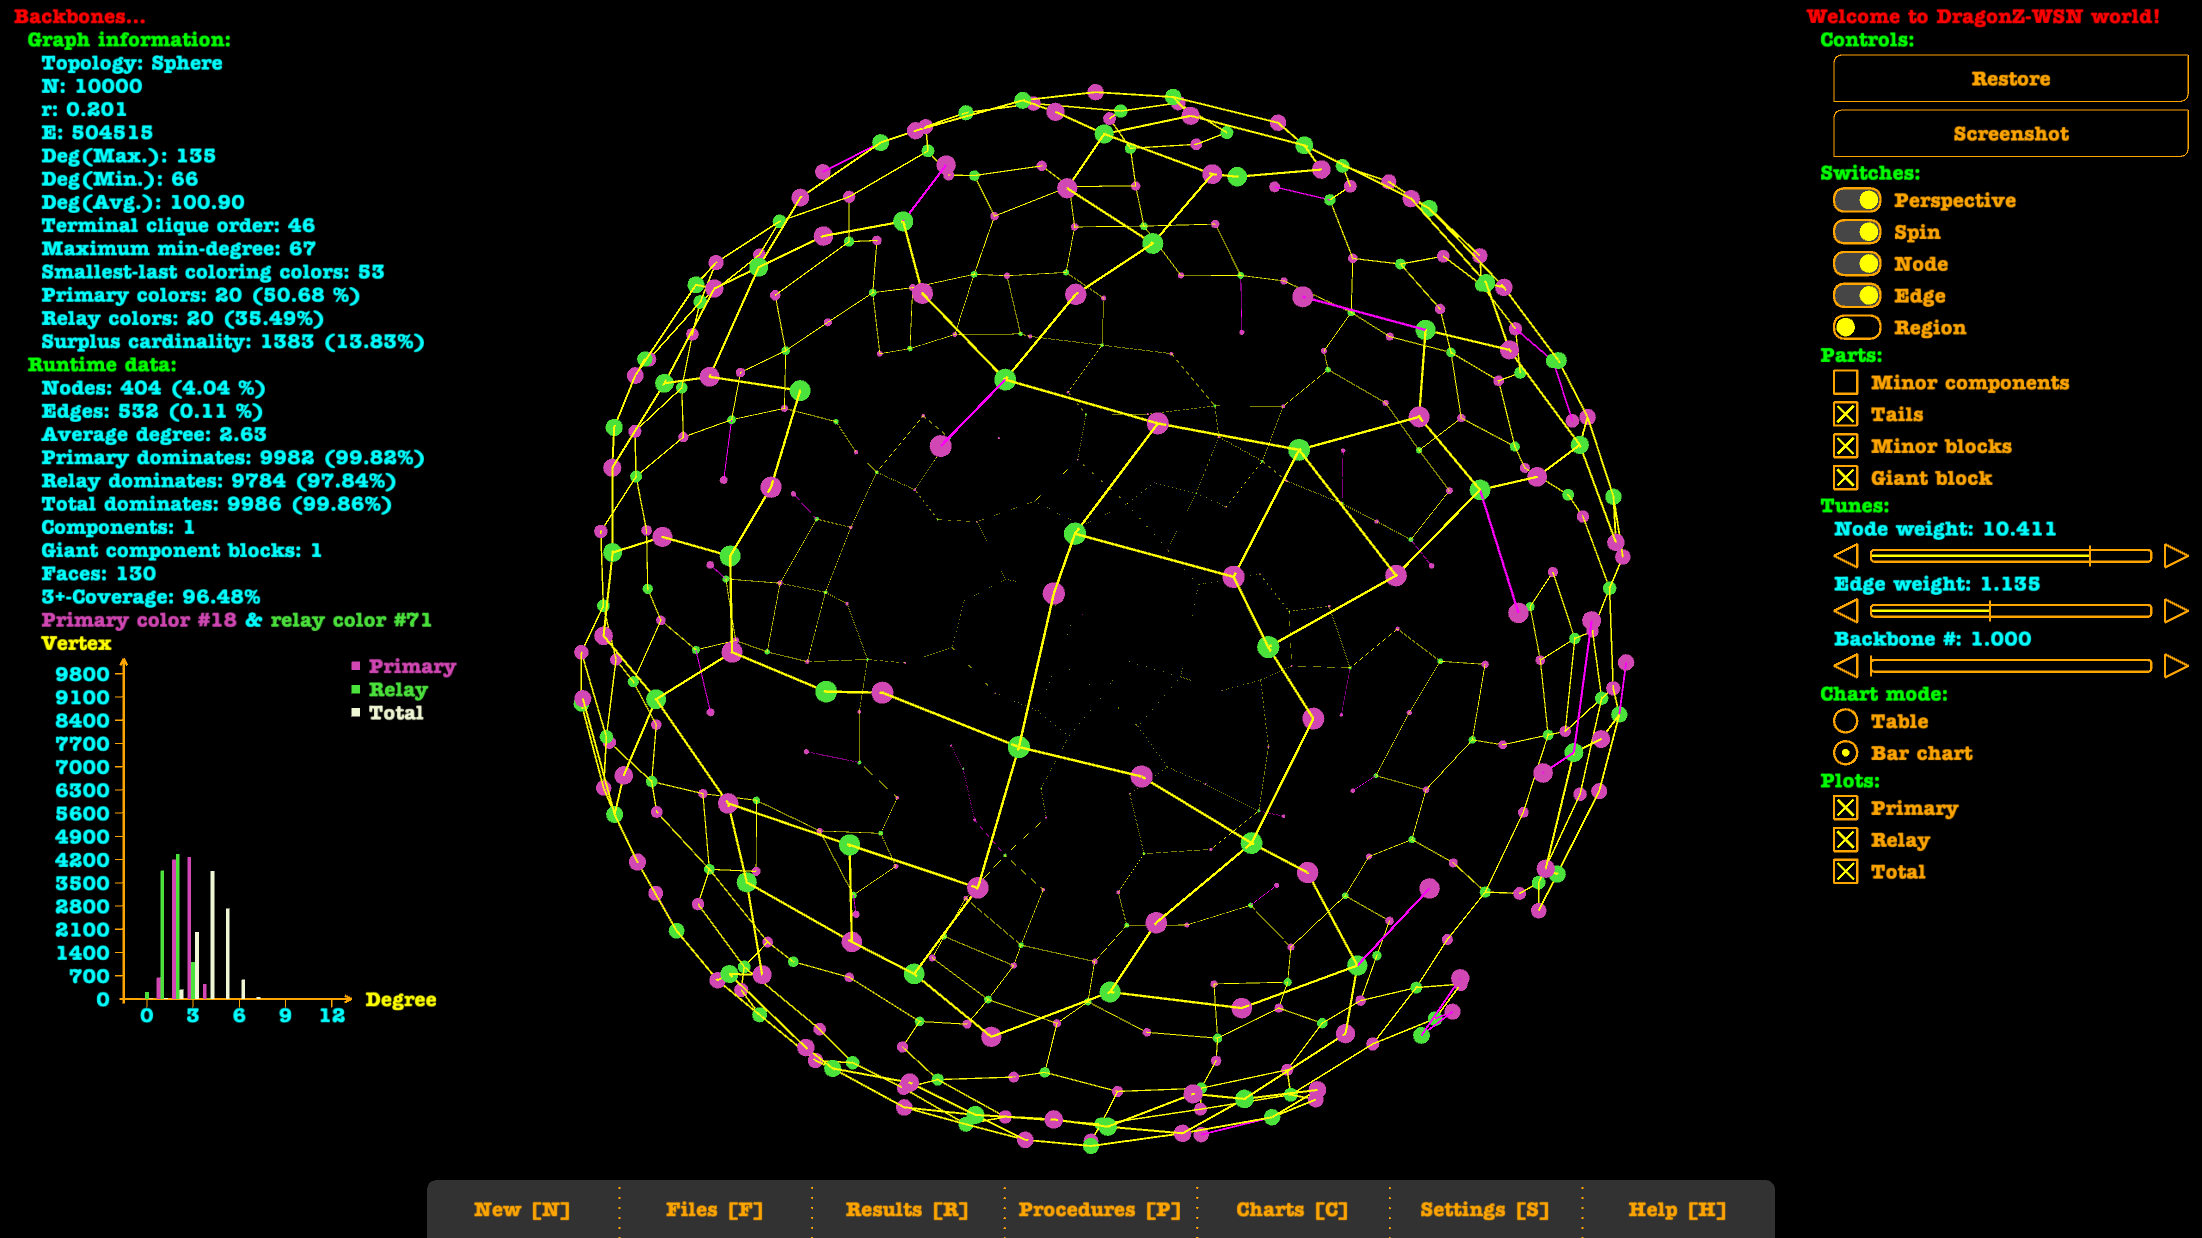
\includegraphics[width=\linewidth]{images/View.png}
	\caption{Program View}
	\label{fig:view}
\end{figure}
There's no specific requirement of screen size since the window is resizable. However, it's preferred to have 16:9 window setup (We tested it in 1920x1080 window size).
\section{Navigation}
There is always a navigation bar (as Figure \ref{fig:navigation} shows) as a dock in the middle bottom of the program window.
 \begin{figure}[htp]
	\centering
	
\includegraphics[width=.8\linewidth]{images/Navigation.png}
	\caption{Navigation Bar}
	\label{fig:navigation}
\end{figure}
Intuitively, the navigation bar supports both mouse control and keyboard control. If a mouse cursor clicked any item of the navigation bar, the corresponding menu will pop up and waiting a further selection of an entry of further action (as Figure \ref{fig:menu} shows).
 \begin{figure}[htp]
	\centering
	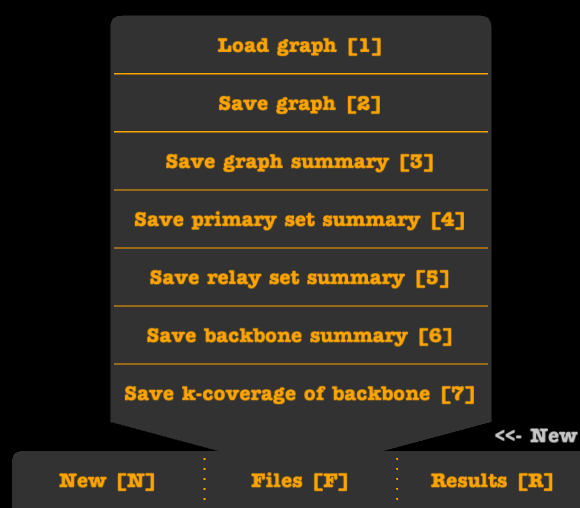
\includegraphics[width=.4\linewidth]{images/Menu.png}
	\caption{Item Menu}
	\label{fig:menu}
\end{figure}
If the mouse cursor clicked somewhere else, the menu disappear. Each item of the bar or any menu entry has a square bracket enclosed character ([*]) as an indicator for keyboard control. The key combination of activating any item is ``\textbf{ALT} + \textbf{*}". For example, ``\textbf{ALT} + \textbf{F}" will pop up the ``Files" menu and furthermore, ``\textbf{ALT} + \textbf{1}" will activate "Load graph" entry and pop up a dialog to load a graph. Each menu also supports Up and Down arrow keys to highlight any entry and press Enter to activate the corresponding action.

The navigation bar contains the following items.
\begin{description}
	\item[New]Start a new project.
  	\item[Files]Load or save a file of graph information.
  	\item[Results]Show graphic final results of computations. 
  	\item[Procedures]Several algorithm procedures of backbone determination.
  	\item[Charts]Show plot charts of some results.
  	\item[Settings]Configure settings of the program.
  	\item[Help]Show documentation or about information.
\end{description}
\section{Create a New Project}
There are three modes of a new project as the``New" menu (Figure \ref{fig:new}) shows.
 \begin{figure}[htp]
	\centering
	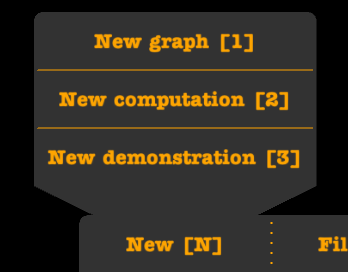
\includegraphics[width=.3\linewidth]{images/New.png}
	\caption{``New" Menu}
	\label{fig:new}
\end{figure}
\begin{enumerate}
	\item``New graph" starts a normal project that requires manually selecting each consecutive algorithmic procedure to partition a \ac{WSN} into virtual backbones.
	\item``New computation" is designed for performing algorithms on a \ac{WSN} of huge amount of nodes. It does not show the graphic procedures and directly complete all algorithmic procedures. However, you are still able to show graphic final results through the ``Results" menu.
	\item``New demonstration" starts a project in a demo mode which automatically performs all consecutive algorithmic procedures on loop.
\end{enumerate}

To start a project, you are required to have a keyboard to input basic information of the expected \ac{WSN}. The input supports mouse and keyboard control. Mouse control is mainly for fixing input typos (use mouse to change the place of input cursor as Figure \ref{fig:input} shows).
 \begin{figure}[htp]
	\centering
	\includegraphics[width=.8\linewidth]{images/input.png}
	\caption{Input}
	\label{fig:input}
\end{figure}
Keyboard control supports Backspace, Delete, Enter and arrow keys. Each information needs an Enter press for confirmation.
\section{Graphic and \ac{UI} control}
As Figure \ref{fig:view} shows, the view of a screen in the program typically can be divided into four parts:
\begin{enumerate}
	\item \textbf{Middle bottom} shows the navigation bar.
	\item \textbf{Left column} shows the runtime data (Screens of ``Chart"s do not have left runtime data column).
	\item \textbf{Right column} is the control area.
	\item \textbf{Center} shows the main graphics.
\end{enumerate}
Screens of ``Results", ``Procedures" and ``Charts" have such view. Other screens have their own dedicated view. ``Files" does not have screen.
\subsection{Main Graphics Control}
Any generated networks and chart plots have 3D control features like moving, zooming and rotating supported by mouse and keyboard control (as Table \ref{tab:3d_control} shows).
\begin{table}[ht]
	\caption{3D Control Features}
	\label{tab:3d_control}
	\begin{tabular}{|c|c|c|}
		\toprule
		Control&Mouse&Keyboard\\
		\midrule
		Moving&right button pressed and drag&arrow keys\\
		\midrule
		Zooming&wheel scroll&'w' and 's' keys\\
		\midrule
		Rotation&left button pressed and drag\footnotemark&'a' and 'd' keys\\
		\bottomrule
	\end{tabular}
\end{table}
\subsection{\ac{UI} Control}
Most \ac{UI} controls are traditional mouse control parts (i.e. buttons, sliders, radios and check boxes) and majority of them support both mouse and keyboard control. The corresponding keyboard controls are pressing the letter key indicated by the bracket ([*]) directly. Some \acp{UI} are controlled by mouse only such as radios and sliders. Text field is the \ac{UI} controlled by keyboard only. In summary, if an \ac{UI} has a bracket ([*]), then it supports the keyboard control by pressing * key. One exception is the check box. The keyboard controls of check boxes are pressing number keys starting from $0$ in the order of the list of check boxes. Keyboard controls are not influence by shift or caps lock keys.
\footnotetext{Chart plots do not support.}
\bibliographystyle{unsrt}
\bibliography{Reference}
\end{document}  